% 建议放在介绍声学记录区间与视频帧代表区间之后、一般聚合公式之前。
为直观说明加权过程，图~\ref{fig:p1_overlap_principle}以三条视觉记录为例。
假设某词的候选时间区间为 $[1.00,1.45]\,\mathrm{s}$，
与三帧代表区间的交叠时长分别为 $0.10\,\mathrm{s}$、$0.20\,\mathrm{s}$ 和 $0.15\,\mathrm{s}$。
其中第二帧没有可用面部特征，因此不参与聚合。
将其余两条记录的交叠时长归一化，得到权重
$0.10/(0.10+0.15)=0.4$ 和 $0.15/(0.10+0.15)=0.6$，
该词的视觉特征即为 $\widehat{\boldsymbol{v}}=0.4\boldsymbol{v}_1+0.6\boldsymbol{v}_3$。
同样的计算规则用于声学记录，两个模态分别归一化并聚合，原有词级文本特征保持不变。

\begin{figure}[htbp]
    \centering
    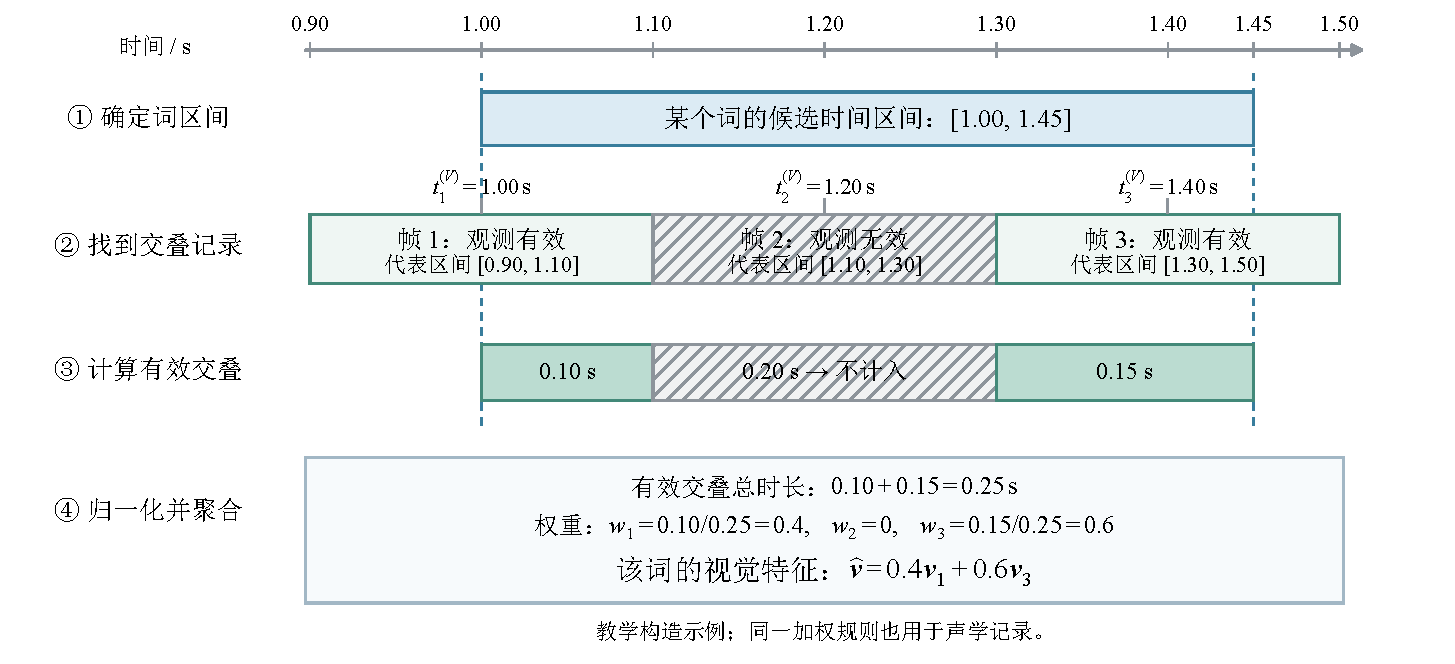
\includegraphics[width=\textwidth]{figures/fig_5_4_overlap_principle.pdf}
    \caption{基于词时间区间的加权聚合示意。
    虚线表示词区间边界，绿色表示有效观测，斜线区域表示无效观测。
    聚合权重由有效观测与词区间的交叠时长归一化得到。
    图中时间与观测状态为教学构造。}
    \label{fig:p1_overlap_principle}
\end{figure}
